%File: main.tex — MIDC, AAAI 2027 anonymous submission
\documentclass[letterpaper]{article}
\usepackage[submission]{aaai2027}
\usepackage[hyphens]{url}
\usepackage{graphicx}
\urlstyle{rm}
\def\UrlFont{\rm}
\usepackage{natbib}
\usepackage{caption}
\frenchspacing
\setlength{\pdfpagewidth}{8.5in}
\setlength{\pdfpageheight}{11in}
\usepackage{algorithm}
\usepackage{algorithmic}
\usepackage{booktabs}
\usepackage{multirow}
\usepackage{amsmath}
\usepackage{amssymb}

\pdfinfo{/TemplateVersion (2027.1)}

\title{MIDC: Calibrated Test-Time Correction for Multi-Subject Identity Collapse}
\author{Anonymous Submission}
\affiliations{Anonymous Institution\\ anonymous@example.com}

\begin{document}
\maketitle

\begin{abstract}
Personalized image generation with multiple subjects suffers from \emph{interaction-induced identity collapse}: as the number of subjects grows, models increasingly merge, swap, or drop identities, even when each subject is provided as a reference image. We introduce \textbf{MIDC}, a training-free, inference-time correction paradigm that treats a \emph{decomposed} verifier as a structured diagnostic signal and routes correction to the most deficient facet. Given a candidate image, a decomposed evaluator scores three facets---existence, appearance, and interaction---and we convert each facet score into a standardized deficit against a calibrated per-facet baseline. A \emph{calibrated routing} mechanism then selects which facet to correct and which action to apply, while a dual-signal diagnosis (facet deficit $+$ subject-level identity similarity) localizes the collapsed subject. Correction proceeds as a propose--verify loop with a guarded acceptance criterion that accepts a revision only if the verifier's overall score does not regress and the collapsed subject's identity similarity strictly improves. On OmniGen2, MIDC reduces Subject Collapse Rate (SCR) to \textbf{0.470} on 4-entity hard cases versus \textbf{0.531} for the retrained state-of-the-art (UMO) and \textbf{0.536} for one-shot generation. Notably, the retrained SOTA is itself a near-tie with one-shot (SCR $\Delta{=}{-}0.005$, DINO identity similarity $\Delta{=}{-}0.0002$ over $500{\times}3$ pairs): retraining the \emph{identity-consistency} axis yields near-zero gain on hard interaction cases, indicating collapse's cause is not on the optimized axis. MIDC's decomposed diagnosis localizes that cause and cheaply repairs it at inference, with 11 of 12 paired bootstrap comparisons significant at $p<0.05$. On FLUX.2-klein-9B, MIDC transfers to a larger, distilled base and improves over one-shot at both 6 and 8 subjects on both metrics ($p\le0.001$) using roughly half the generations of best-of-8; against best-of-8 itself the \emph{aggregate} difference is not significant, because MIDC deliberately acts on only the $28$--$33\%$ of rows its calibrated deficit flags---on those rows it cuts SCR by $23.8\%$ and beats best-of-8 decisively. A blind human study independently corroborates the existence result: labelers prefer MIDC over UMO 84.6\% of the time ($p{=}4{\times}10^{-7}$). Ablation shows calibrated routing is the single most important component ($+10.3\%$ SCR without it); dual-signal diagnosis contributes the smallest marginal gain ($+1.3\%$ on 4-entity cases), and we conjecture it matters more at higher subject counts.
\end{abstract}

\begin{figure}[t]
\centering

\includegraphics[width=0.92\columnwidth]{figures/teaser.pdf}
\caption{Interaction-induced identity collapse, 8-subject FLUX.2-klein-9B (\texttt{hard\_048829}); both panels share a seed, so they differ only in method. Each cell under an image is one subject and carries its DINOv2 similarity to the reference, red when below the $0.5$ threshold SCR is defined by; SCR is the fraction of red cells. One-shot collapses 6 of the 8 subjects (SCR $0.75$); MIDC collapses 1 (SCR $0.125$).}
\label{fig:teaser}
\end{figure}

\section{Introduction}

Personalized text-to-image generation has progressed rapidly, with subject-driven methods~\citep{gal2022image,ruiz2023dreambooth,kumari2023multi,ye2023ip} now able to condition on reference images of specific subjects. Yet a persistent failure mode remains: when a prompt asks for \emph{several} subjects at once---especially in interaction---models frequently produce images where one subject's identity leaks into another, a subject is dropped entirely, or identities merge into an ambiguous composite. We call this \emph{interaction-induced identity collapse}, and it worsens monotonically with the number of subjects (Figure~\ref{fig:teaser}): in our experiments, the Subject Collapse Rate (SCR) of one-shot FLUX.2-klein-9B rises from $0.615$ at 6 subjects to $0.671$ at 8 subjects.

Existing remedies fall into two camps. \emph{Retraining-based} approaches~\citep{she2025mosaic,chen2025xverse,wang2025psr,he2024uniportrait} fine-tune on multi-identity data, but they are bound to a specific base model, expensive to train, and---as we show---barely improve over one-shot generation on hard interaction cases: UMO~\citep{cheng2025umo}, a retrained SOTA, scores SCR $0.531$ vs.\ one-shot $0.536$ on our hard 4-entity split (a near-tie, with DINO identity similarity $\Delta{=}{-}0.0002$ over $500{\times}3$ pairs---marginally better on SCR, marginally worse on DINO). This is not a failure of training in general---it is evidence that the axis retraining optimizes (identity consistency) is \emph{not} where interaction-induced collapse bites, which is precisely why the collapse is inference-diagnosable and cheaply partially repairable. \emph{Training-free} selection approaches such as best-of-$N$~\citep{snell2024testtime} spend extra inference compute but apply \emph{no structured diagnosis}: they pick the highest-scoring candidate without knowing \emph{what} is wrong or \emph{which subject} collapsed, so gains are modest and compute-inefficient.

We argue that the missing ingredient is a \emph{structured, decomposed verifier} that separates distinct failure facets. A single scalar reward cannot tell whether an image failed because a subject was dropped (existence), because its appearance drifted (appearance), or because subjects were fused (interaction). A decomposed evaluator that scores each facet independently exposes \emph{which} facet is deficient, enabling targeted correction rather than blind re-sampling.

We introduce \textbf{MIDC} (Multi-subject Interaction Diagnosis and Correction), a training-free, inference-time paradigm built around three ideas:
\begin{itemize}
\item \textbf{Calibrated deficit routing.} A decomposed evaluator scores existence, appearance, and interaction. We convert each facet score to a standardized deficit $(\mathrm{median}_d - s_d)/\mathrm{scale}_d$ against a frozen per-facet calibration, and route correction to the facet with the largest deficit. Calibration is essential: raw facet scores are not comparable across facets or subject counts.
\item \textbf{Dual-signal diagnosis.} The facet deficit tells us \emph{what} is wrong; a subject-level identity-similarity signal (DINOv2~\citep{oquab2023dinov2} against each reference, made detection-aware with Grounding-DINO~\citep{liu2023grounding}) tells us \emph{which} subject collapsed. Together they target the right subject with the right action.
\item \textbf{Propose--verify with guarded acceptance.} Each step applies an action from a small portfolio (targeted reference reordering, layout hint, facet-specific prompt rewrite) and is accepted only if the verifier's overall score does not regress and the collapsed subject's identity similarity improves---preventing the correction loop from drifting.
\end{itemize}

Crucially, MIDC is \emph{training-free} and \emph{model-agnostic}: it treats the generator as a black box and only requires a decomposed scorer. We instantiate it on two base models---OmniGen2~\citep{wu2025omnigen2} and FLUX.2-klein-9B~\citep{blackforest2025flux2}---using a Qwen3.5-4B-based decomposed evaluator (MIE) as the verifier, and report a DINOv2-based Subject Collapse Rate as the judge. That judge is independent of the verifier but \emph{not} of the loop---MIDC also consults DINOv2 per-subject similarity when diagnosing and accepting---so we quantify the exposure in \emph{Limitations} rather than claim independence.

Our contributions:
\begin{enumerate}
\item We formalize \emph{interaction-induced identity collapse} and show it worsens with subject count---a problem retraining alone does not solve.
\item We propose \emph{calibrated deficit routing} on a decomposed verifier as the core mechanism for training-free multi-subject correction, and ablate it as the single most important component ($+10.3\%$ SCR without it).
\item \textbf{Finding:} on hard interaction cases, retraining the identity-consistency axis yields near-zero gain---the retrained SOTA (UMO) is a near-tie with one-shot (SCR $0.531$ vs $0.536$, DINO $\Delta{=}{-}0.0002$ over $500{\times}3$). This indicates interaction-induced collapse's cause is \emph{not} on the axis retraining optimizes, which is why it is inference-diagnosable and cheaply partially repairable. Across 500 tasks $\times$ 3 seeds on OmniGen2, MIDC beats UMO on both SCR and DINO identity similarity at $p=0.0$ (11 of 12 MIDC-vs-baseline comparisons significant).
\item On FLUX.2-klein-9B, MIDC generalizes to a larger, distilled model, significantly improving over one-shot at both 6 and 8 entities on both metrics at a fraction of best-of-8's compute. We further show the gain is \emph{selective} rather than diffuse: MIDC acts on only the $28$--$33\%$ of rows its calibrated deficit flags, cuts SCR by $23.8\%$ on those, and is a measurable no-op on the rest.
\end{enumerate}

\section{Related Work}

\paragraph{Subject-driven generation.} Personalization methods condition a diffusion model on a few reference images of a subject. DreamBooth~\citep{ruiz2023dreambooth} and Custom Diffusion~\citep{kumari2023multi} fine-tune weights; IP-Adapter~\citep{ye2023ip}, InstantID~\citep{wang2024instantid}, and PhotoMaker~\citep{li2024photomaker} add lightweight conditioning modules; ControlNet~\citep{zhang2023adding} adds spatial conditioning. Foundational text-to-image models~\citep{ramesh2022hierarchical} established the CLIP-latent conditioning paradigm. These are largely single-subject; multi-subject extensions~\citep{xiao2023fastcomposer,gu2024mix,he2024uniportrait,she2025mosaic,chen2025xverse,wang2024ms,he2025anystory} require retraining and are tied to a specific base model.

\paragraph{Multi-subject identity consistency.} MOSAIC~\citep{she2025mosaic}, XVerse~\citep{chen2025xverse}, UniPortrait~\citep{he2024uniportrait}, PSR~\citep{wang2025psr}, MS-Diffusion~\citep{wang2024ms}, and AnyStory~\citep{he2025anystory} improve multi-identity fidelity through dedicated training data and identity-preserving losses; FocusDPO~\citep{jin2025focusdpo} aligns multi-subject generation with preference optimization, and InteractCustom~\citep{xu2025interactcustom} targets human-object interaction. Recent benchmarks~\citep{borse2025multihuman,oshima2025multibanana} quantify multi-identity fidelity at scale. UMO~\citep{cheng2025umo} is a retrained SOTA that applies a multi-to-multi matching reward (ReReFL) to OmniGen2~\citep{wu2025omnigen2} via a context-refiner LoRA. We show these methods do not resolve \emph{interaction-induced} collapse and can even underperform one-shot generation on hard splits.

\paragraph{Training-free test-time methods.} Best-of-$N$ selection~\citep{snell2024testtime,cobbe2021gsm8k} and self-refinement~\citep{madaan2023selfrefine} spend extra inference compute but use a scalar reward. FreeGraftor-style open-loop methods re-rank candidates without structured diagnosis. MIDC differs by using a \emph{decomposed} verifier to route correction to a specific facet and subject, yielding larger gains per unit of compute.

\paragraph{Decomposed evaluation.} Benchmarks such as DreamBench~\citep{ruiz2023dreambooth}, DreamBench++~\citep{peng2024dreambench++}, and T2I-CompBench~\citep{huang2023t2i} evaluate text-to-image alignment along multiple axes. Human-preference reward models~\citep{xu2023imagereward,kirstain2023pick,wu2023human} and reference-based similarity metrics~\citep{radford2021learning,deng2019arcface,wang2004image,hore2010image,wang2003multiscale} give scalar scores but do not decompose \emph{which} facet failed for \emph{which} subject. We build on MIE~\citep{anon2025mibe}, a decomposed multi-subject evaluator that scores existence, appearance, and interaction separately. MIE is a lightweight reference-conditioned evaluator trained on a 60K-pair LLM-labeled Silver Set, reaching $0.922$ pairwise agreement with human preference on a 4K-pair double-blind Gold Set ($0.884$ on unseen generators). We use MIE as a \emph{verifier} for correction rather than only for evaluation, and report headline metrics from a separate DINOv2-based Subject Collapse Rate; \emph{Limitations} audits what that separation does and does not buy.

\section{Method}

MIDC is a training-free, inference-time correction loop. Given a prompt, a set of subject reference images, and a black-box generator $G$, MIDC produces a corrected image by iteratively diagnosing facet deficits, targeting the weakest subject, applying a corrective action, and accepting the result only if it strictly improves the targeted facet without collateral damage. Figure~\ref{fig:pipeline} illustrates the pipeline.

\begin{figure}[t]
\centering
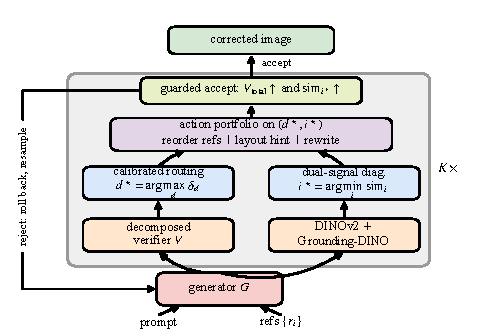
\includegraphics[width=0.95\columnwidth]{figures/pipeline.pdf}
\caption{MIDC. The grey block runs for $K$ correction steps. A candidate from the black-box generator is scored twice: the decomposed verifier $V$ gives per-facet scores, and detection-aware DINOv2 gives per-subject identity. \emph{Calibrated routing} picks the facet with the largest standardized deficit $d^\star$, \emph{dual-signal diagnosis} picks the weakest subject $i^\star$, and the portfolio acts on that pair; a revision is kept only if the verifier total and $\mathrm{sim}_{i^\star}$ both improve, else it is rolled back and resampled. On \texttt{hard\_058139} this routes to interaction ($\delta{=}{+}0.69$, over $+0.54$ and $-1.08$) and to $s_4$ (undetected, $\mathrm{sim}{=}{-}1$); step~1 is \emph{rejected} (total $-0.63{\to}{-}0.77$), step~2 accepted (total $-0.35$, all four subjects recovered, SCR $0.00$).}
\label{fig:pipeline}
\end{figure}

\subsection{Decomposed Verifier}
\label{sec:verifier}

Let a candidate image $I$ be scored by a decomposed evaluator $V$ along three facets:
\[
\mathbf{s} = V(I, \text{prompt}, \text{refs}) = \{s_{\mathrm{ex}}, s_{\mathrm{ap}}, s_{\mathrm{int}}\},
\]
where $s_{\mathrm{ex}}$ measures subject existence (are all subjects present?), $s_{\mathrm{ap}}$ measures appearance fidelity (does each present subject match its reference?), and $s_{\mathrm{int}}$ measures interaction correctness (are subjects arranged as the prompt asks?). We instantiate $V$ with a Qwen3.5-4B-based~\citep{yang2024qwen2} multi-subject evaluator fine-tuned via LoRA~\citep{hu2021lora,unsloth2024} to emit per-facet scores.

\subsection{Calibrated Deficit Routing}
\label{sec:routing}

Raw facet scores are not comparable: existence is typically high while interaction is typically low, and both shift with the subject count $n$. We calibrate against a frozen baseline distribution. For each facet $d$ and subject count $n$, we precompute a median $\mathrm{median}_d^{(n)}$ and scale $\mathrm{scale}_d^{(n)}$ over a calibration set of one-shot generations. The standardized deficit of facet $d$ on image $I$ with $n$ subjects is
\[
\delta_d(I) = \frac{\mathrm{median}_d^{(n)} - s_d(I)}{\mathrm{scale}_d^{(n)}},
\]
with larger $\delta_d$ meaning worse deficit relative to the typical one-shot image. \textbf{Routing} selects the facet with the largest deficit:
\[
d^\star = \arg\max_d \delta_d(I).
\]
This is the facet MIDC will correct. Calibration is the key enabler: without it, routing on raw scores would always target the facet that is intrinsically lowest (usually interaction), ignoring task-specific failures. Our ablation (\emph{Ablation}) confirms calibrated routing is the single most important component ($+10.3\%$ SCR when removed).

\subsection{Dual-Signal Diagnosis}
\label{sec:dual}

Knowing \emph{which facet} is deficient is not enough; we must know \emph{which subject} collapsed. We compute a subject-level identity similarity $\rho_i$ for each reference $i$ using DINOv2~\citep{oquab2023dinov2} features, made detection-aware via Grounding-DINO~\citep{liu2023grounding}: we first detect subjects in $I$, match each detection to a reference by feature similarity, and set $\rho_i$ to the best-match similarity, or $-1$ if subject $i$ is not detected at all---so an undetected subject always sorts below a merely degraded one. The \emph{weak subject} is
\[
i^\star = \arg\min_i \rho_i.
\]
The dual signal $(d^\star, i^\star)$---facet deficit plus weak subject---targets the correction at the right problem on the right subject.

\subsection{Action Portfolio}
\label{sec:portfolio}

At each correction step we instantiate up to three distinct actions conditioned on $d^\star$, generate proposals for \emph{each}, and keep the best---an action-space search, not a single sampled edit, which is where most of MIDC's extra generations go:
\begin{itemize}
\item \textbf{Targeted reference reordering} (for $d^\star\in\{\mathrm{ex},\mathrm{ap}\}$): move reference $i^\star$ to the front and duplicate it, biasing the generator's cross-attention toward the weak subject.
\item \textbf{Layout hint} (for $d^\star=\mathrm{int}$): prepend a spatial layout description to the prompt to enforce the requested arrangement.
\item \textbf{Facet-specific prompt rewrite} (for any $d^\star$): append an explicit instruction targeting the deficient facet (e.g., ``ensure every subject is fully visible'').
\end{itemize}
We draw $K_p$ proposals per action; the candidate kept is the one that most improves the diagnosed subject's identity similarity.

\subsection{Guarded Acceptance}
\label{sec:accept}

A proposal $I'$ is accepted only if the verifier's \emph{overall} score does not regress \emph{and} the collapsed subject's identity similarity strictly improves:
\[
\begin{aligned}
\mathrm{accept}(I') \iff\ & \big(V_{\mathrm{total}}(I') > V_{\mathrm{total}}(I)\big) \\[-1pt]
 &\wedge\ \big(\mathrm{sim}_{i^\star}(I') > \mathrm{sim}_{i^\star}(I)\big),
\end{aligned}
\]
where $V_{\mathrm{total}}$ is the verifier's aggregate score and $\mathrm{sim}_{i^\star}$ is the DINOv2 identity similarity of the weak subject $i^\star$ identified by dual-signal diagnosis. We use a \emph{relaxed} acceptance that drops an explicit per-subject collateral check: emphasizing one subject inherently trades off attention from others, so requiring every other subject's similarity not to dip rejects nearly every correction, while $V_{\mathrm{total}}$ already guards overall quality. The total-improvement margin is strict ($\tau_{\mathrm{total}}{=}0$). The loop runs $K$ correction steps and always keeps the best image seen so far by verifier total. Throughout, $K$ counts correction steps and $K_p$ proposals per action.

\subsection{Algorithm}

\begin{algorithm}[ht]
\caption{MIDC inference (one task)}
\begin{algorithmic}[1]
\STATE \textbf{Input:} prompt, refs $\{r_i\}$, generator $G$, verifier $V$, calibration $\{\mathrm{median}_d^{(n)}, \mathrm{scale}_d^{(n)}\}$, steps $K$, proposals $K_p$
\STATE Generate $K_p$ initial candidates $\{I_j\}$ via $G$; set $I \leftarrow \arg\max_j V(I_j).\text{total}$
\FOR{step $= 1 \dots K$}
  \STATE $\mathbf{s} \leftarrow V(I)$; $\delta_d \leftarrow (\mathrm{median}_d^{(n)} - s_d)/\mathrm{scale}_d^{(n)}$
  \STATE $d^\star \leftarrow \arg\max_d \delta_d$ \hfill // calibrated routing
  \STATE $\rho_i \leftarrow \mathrm{DINOv2Sim}(I, r_i)$; $i^\star \leftarrow \arg\min_i \rho_i$ \hfill // dual-signal diagnosis
  \STATE Sample actions $\mathcal{A}$ from portfolio conditioned on $d^\star$
  \STATE Generate $K_p$ proposals per action; pick best $I'$ by $V.\text{total}$
  \IF{$\mathrm{accept}(I')$}
    \STATE $I \leftarrow I'$
  \ENDIF
\ENDFOR
\STATE \textbf{return} $I$
\end{algorithmic}
\end{algorithm}

\section{Experiments}

\subsection{Setup}

\paragraph{Models.} We instantiate MIDC on two base generators: (i) \textbf{OmniGen2}~\citep{wu2025omnigen2}, a native multi-reference model (up to 5 references), and (ii) \textbf{FLUX.2-klein-9B}~\citep{blackforest2025flux2}, a 9B step-distilled model supporting up to 8 reference images. MIDC treats both as black boxes.

\paragraph{Verifier.} The decomposed verifier $V$ is a Qwen3.5-4B model~\citep{yang2024qwen2} fine-tuned via LoRA~\citep{hu2021lora,unsloth2024} to emit existence/appearance/interaction scores. Calibration statistics $\{\mathrm{median}_d^{(n)}, \mathrm{scale}_d^{(n)}\}$ are frozen from a one-shot calibration set disjoint from all evaluation splits.

\paragraph{Benchmarks.} We use the MIB-Gold hard splits from MIBE~\citep{anon2025mibe}: (i) a 500-task OmniGen2 split (250 hard 4-entity $+$ 250 easy 2-entity) and (ii) FLUX.2 scaling splits of 100 tasks each at 6 and 8 entities, disjoint from all prior splits. Tasks emphasize interaction and occlusion.

\paragraph{Baselines.} On OmniGen2 we compare to \textbf{one\_shot} (single generation), \textbf{best\_of\_n} (generate $N{=}8$ candidates, pick best by verifier total; a stronger-compute baseline at $\sim 2\times$ MIDC's generations), and \textbf{UMO}~\citep{cheng2025umo} (retrained SOTA for multi-identity consistency, applied to OmniGen2~\citep{wu2025omnigen2} via a context-refiner LoRA of rank $512$ that fine-tunes both the context refiner and the main transformer blocks). UMO uses its officially recommended \texttt{image\_guidance\_scale}$=2.0$; MIDC uses $2.5$ for OmniGen2.\footnote{We verified the UMO LoRA loads correctly and is not a silent no-op over base OmniGen2: a key-match check returns zero unexpected keys (all 304 LoRA keys load), and a same-seed pixel-diff between base and UMO yields a mean absolute difference of $10.44$ (on $0$–$255$), confirming substantial effect. Details in the supplementary. For full disclosure, the UMO runner also uses a longer negative prompt (naming ``extra limbs, fused fingers'') and does not pass \texttt{max\_pixels}, following UMO's official inference config; our one\_shot/MIDC runner uses a shorter negative prompt and \texttt{max\_pixels}$=1024^2$. We keep each method's own recommended setting rather than equalizing, but this is not a cosmetic difference: it roughly halves output sharpness (\emph{Main Results}), which we quantify and control for rather than leave implicit.} On FLUX.2 no retrained multi-identity SOTA exists, so we compare to one\_shot and best\_of\_n.

\paragraph{Metrics.} Headline metrics are \emph{independent} of the verifier $V$ to avoid circularity: (i) \textbf{Subject Collapse Rate (SCR)}---detection-aware, DINOv2-based; lower is better; (ii) \textbf{DINO identity similarity}---mean DINOv2 similarity of detected subjects to their references; higher is better. We also report verifier scores for diagnosis. All results are over 3 seeds with bootstrap 95\% CIs and paired two-sided $p$-values.

\paragraph{Implementation.} MIDC uses $K{=}2$ correction steps, $K_p{=}2$ proposals per action, 3 actions per step, and relaxed guarded acceptance ($\tau_{\mathrm{total}}{=}0$; per-subject collateral dropped). Reference reordering uses front-duplication of the weak subject. FLUX.2 uses 4 inference steps (step-distilled) with guidance 4.0.

\paragraph{Infrastructure.} All generation and scoring runs on NVIDIA A100 GPUs (one per evaluation shard, four in parallel) with PyTorch 2.6.0 (CUDA 12.4), \texttt{diffusers} 0.39.0, \texttt{transformers} 4.51.3. The OmniGen2 main run dominates cost at ${\approx}33$ GPU-hours per shard. No weights are trained anywhere; every reported method is inference-only.

\subsection{Main Results: OmniGen2}
\label{sec:main}

Table~\ref{tab:main} reports SCR and DINO on the 500-task OmniGen2 split over 3 seeds. MIDC achieves the lowest SCR and highest DINO on both difficulty slices.

\begin{table}[ht]
\centering
\footnotesize
\setlength{\tabcolsep}{3.5pt}
\caption{OmniGen2 hard 4-entity ($n{=}250$). SCR and DINO are 3-seed per-task means with 95\% bootstrap CIs; CLIP-I and CLIP-T are seed 0 ($n{=}500$ over both slices). SCR and DINO both derive from the same DINOv2 similarity array, so CLIP-I is the only identity number here independent of that pipeline, and CLIP-T is scored against the prompt \emph{as requested}---it tests whether MIDC's prompt rewriting drifts from the ask.}
\label{tab:main}
\begin{tabular}{lcccc}
\toprule
& SCR $\downarrow$ & DINO $\uparrow$ & CLIP-I $\uparrow$ & CLIP-T $\uparrow$ \\
\midrule
one\_shot & 0.536 \tiny[.513,.558] & 0.455 \tiny[.441,.469] & 0.656 & 0.317 \\
best\_of\_n & 0.492 \tiny[.465,.518] & 0.492 \tiny[.476,.508] & 0.657 & \textbf{0.323} \\
UMO & 0.531 \tiny[.509,.553] & 0.455 \tiny[.441,.469] & \textbf{0.666} & 0.316 \\
\textbf{MIDC} & \textbf{0.470} \tiny[.448,.491] & \textbf{0.509} \tiny[.496,.523] & 0.662 & 0.321 \\
\bottomrule
\end{tabular}
\end{table}

\paragraph{Significance.} Paired bootstrap over 3-seed-averaged per-task scores. On hard\_4, MIDC vs.\ UMO: SCR $-0.061$ [$-0.081,-0.041$], $p{=}0.0$ (win/tie/loss $135/51/64$); DINO $+0.054$ [$0.042,0.067$], $p{=}0.0$. MIDC vs.\ best\_of\_n: SCR $-0.022$ [$-0.044,+0.000$], $p{=}0.056$ (\emph{not} significant); DINO $+0.017$, $p{=}0.004$. SCR is discrete (multiples of $1/n$) so ties are frequent, and against best\_of\_n the win \emph{count} is below $50\%$, consistent with the borderline mean. Overall \textbf{11 of 12} MIDC-vs-baseline comparisons reach $p<0.05$; the sole exception is that best\_of\_n SCR comparison, which we do not claim. Notably, the retrained SOTA (UMO) is the \emph{worst} or near-worst method on every slice---retraining alone does not resolve interaction-induced collapse. Figure~\ref{fig:umo} shows what this looks like on a single task.

\paragraph{The UMO comparison is not a sharpness artifact.} UMO's official runner produces systematically softer images: on a random 120-task sample it is softer than one\_shot on \textbf{120 of 120} tasks (median Laplacian variance $456$ vs.\ $878$, sign test $p{=}1.2{\times}10^{-12}$), while best\_of\_n ($845$) and MIDC ($832$) match one\_shot. Since SCR and DINO are both DINOv2-derived, softness rather than identity could be driving them. A sharpness-matched control settles it: blurring one\_shot down to UMO's level ($898{\to}422$ median, $n{=}150$) costs only $+0.013$ SCR and $-0.008$ DINO---\emph{larger} than the whole UMO-vs-one\_shot difference we report ($-0.005$, $-0.0002$) and pointing the other way, so correcting for sharpness would make UMO look marginally \emph{better}. The near-tie is robust, and if anything conservative.

\paragraph{An identity signal independent of DINOv2.} SCR is our per-subject DINOv2 similarity array thresholded at $0.5$ and DINO is its mean, so the two are one measurement reported twice (Pearson $r{=}{-}0.81$ across $7860$ records), not independent evidence. Table~\ref{tab:main} therefore also reports CLIP-I (ViT-L/14 image--reference similarity) and CLIP-T (image vs.\ the \emph{originally requested} prompt, never MIDC's rewrite). \textbf{MIDC does not buy subject presence by drifting from the prompt}---the objection its prompt rewriting and reference duplication invite---since CLIP-T \emph{improves} over one\_shot and UMO. CLIP-I, however, puts UMO marginally ahead of MIDC, the one place any metric does: consistent with the sharpness result above, as CLIP features are less blur-sensitive than DINOv2 and so penalise UMO's softer output less. We report this rather than resolve it: on the hard split the identity verdict is metric-dependent, and only the existence axis agrees across DINOv2, CLIP and human labelers.


\paragraph{On the 2-subject split.} The easy\_2 slice gives the same ordering (SCR $0.438$ for MIDC vs.\ $0.467$ best\_of\_n, $0.511$ one\_shot, $0.517$ UMO) but we do not lean on it: at $n{=}2$ SCR takes only $\{0,0.5,1\}$, so per-task CIs are coarse. The ``collapse worsens with subject count'' claim rests instead on the FLUX.2 scaling study (\emph{FLUX.2 Scaling}).

\begin{figure}[t]
\centering
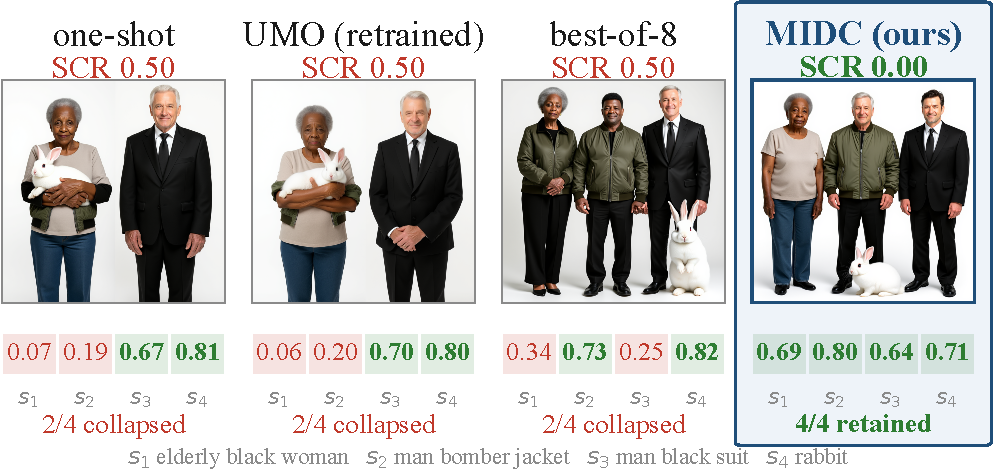
\includegraphics[width=0.97\columnwidth]{figures/umo_qualitative.pdf}
\caption{The retrained-SOTA comparison, OmniGen2 hard 4-entity task \texttt{hard\_046947}, seed 0. Cells are the per-subject DINOv2 similarities that SCR thresholds at $0.5$; red cells are collapsed subjects, so SCR is the fraction of red and the reader can count it rather than take it on trust. One-shot and UMO fail identically: the bomber jacket bleeds onto the elderly woman and its wearer is dropped ($s_1{=}0.07/0.06$, $s_2{=}0.19/0.20$). Best-of-8 recovers him but loses the black-suit man ($s_3{=}0.25$). Only MIDC clears all four. The task is one of $60$ of $250$ hard 4-entity tasks where MIDC is no worse than every baseline on every seed, and is \emph{not} the largest-margin one; its 3-seed SCR means are $0.58$, $0.58$, $0.50$, $0.33$.}
\label{fig:umo}
\end{figure}

\subsection{FLUX.2 Scaling: 6 and 8 Subjects}
\label{sec:scaling}

Table~\ref{tab:flux2} tests generalization to a larger, distilled base. MIDC has the best point estimate on SCR and DINO at both 6 and 8 entities; we quantify below which differences are statistically supported.

\begin{table}[ht]
\centering
\small
\caption{FLUX.2-klein-9B, 3 seeds, n=100 tasks per cell. 95\% bootstrap CI.}
\label{tab:flux2}
\begin{tabular}{lcc}
\toprule
& 6 entities & 8 entities \\
\midrule
\multicolumn{3}{l}{\textit{SCR (lower better)}} \\
\midrule
one\_shot & 0.615 [0.589, 0.639] & 0.671 [0.648, 0.693] \\
best\_of\_8 & 0.607 [0.578, 0.637] & 0.645 [0.616, 0.673] \\
\textbf{MIDC (ours)} & \textbf{0.580 [0.551, 0.607]} & \textbf{0.630 [0.603, 0.657]} \\
\midrule
\multicolumn{3}{l}{\textit{DINO (higher better)}} \\
\midrule
one\_shot & 0.393 [0.373, 0.412] & 0.346 [0.329, 0.363] \\
best\_of\_8 & 0.408 [0.387, 0.428] & 0.369 [0.349, 0.390] \\
\textbf{MIDC (ours)} & \textbf{0.428 [0.408, 0.448]} & \textbf{0.379 [0.358, 0.398]} \\
\bottomrule
\end{tabular}
\end{table}

\paragraph{Significance.} Paired bootstrap over 3-seed-averaged per-task scores ($n{=}100$ per cell). \textbf{Against one\_shot all four comparisons are significant}: SCR $-0.035$ [$-0.053,-0.018$] at 6 entities, $-0.041$ [$-0.066,-0.017$] at 8 ($p{\le}0.001$); DINO $+0.035$ [$+0.024,+0.048$] and $+0.033$ [$+0.019,+0.048$] ($p{=}0.000$). \textbf{Against best\_of\_8 the aggregate differences are mostly not significant}: SCR $p{=}0.067$ at 6 entities and $p{=}0.312$ at 8; DINO $+0.021$ [$+0.007,+0.034$], $p{=}0.002$ at 6 but $p{=}0.233$ at 8. We therefore claim a significant improvement over the base generator, and \emph{not} an aggregate win over best-of-8. \emph{Selective Correction} shows why: MIDC is a selective fixer, so its aggregate mixes a large gain on the minority of rows it acts on with a deliberate no-op on the rest.

\paragraph{Collapse worsens with subject count.} One\_shot SCR rises from $0.615$ (6 entities) to $0.671$ (8). MIDC's gap to one\_shot is nominally larger at 8 ($-0.041$) than at 6 ($-0.035$), but the intervals overlap and we did not test the interaction, so we do not claim it widens.

\paragraph{Compute.} MIDC is adaptive: it stops as soon as the calibrated deficit falls below a threshold, so it spends extra generations only on hard tasks. Averaged over all tasks it issues \textbf{4.6} generator calls on OmniGen2 and \textbf{4.3} on FLUX.2 8-entity, against a fixed $8.0$ for best-of-8 and $1.0$ for one\_shot and UMO. MIDC therefore reaches its results at roughly \emph{half} best-of-8's generation budget; one\_shot and UMO are cheaper still but carry no diagnostic structure and, as shown above, no advantage on hard interaction cases.

\begin{figure}[t]
\centering
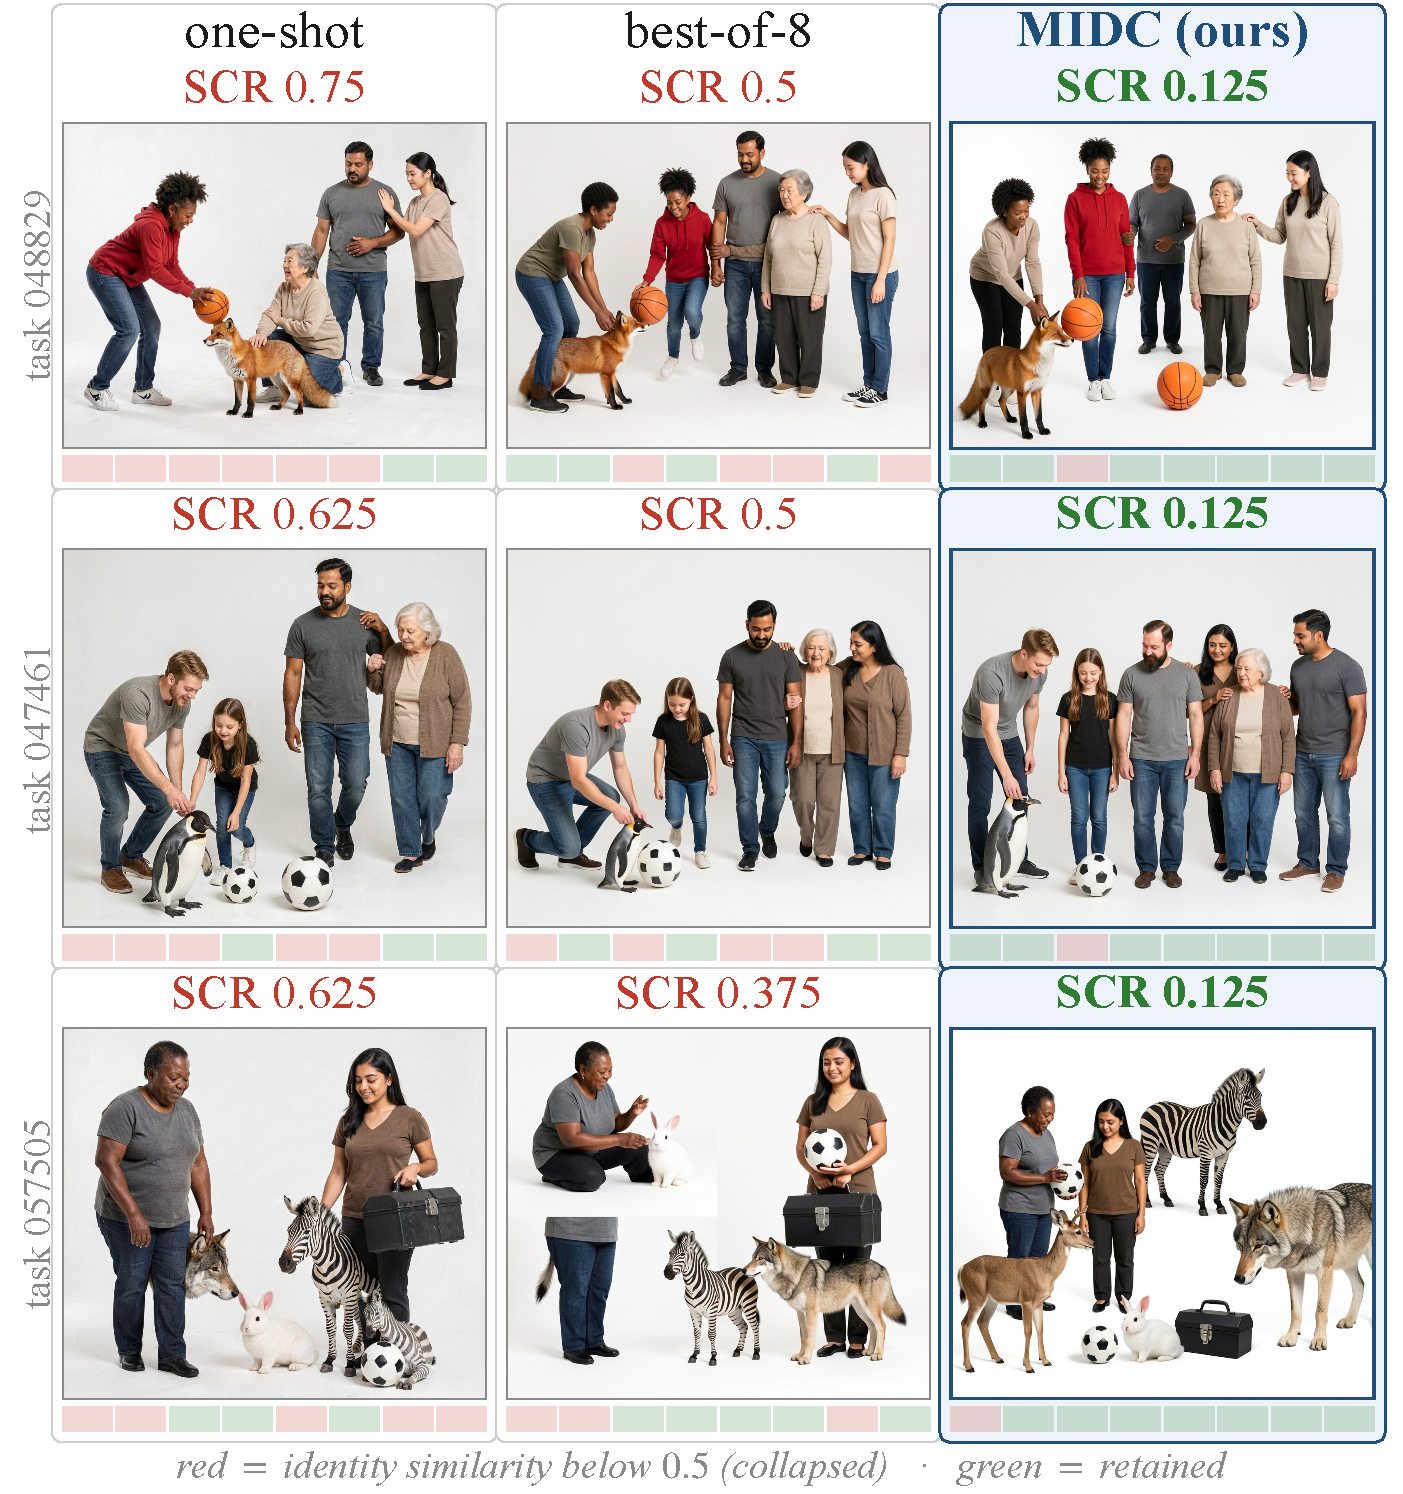
\includegraphics[width=0.90\columnwidth]{figures/results_grid.pdf}
\caption{Qualitative comparison on FLUX.2-klein-9B, 8-subject tasks. Columns: one-shot, best-of-8 ($\sim 2\times$ MIDC's compute), MIDC; \emph{each row is a single seed}, so the three panels differ only in method. Cells are per-subject identity, red $=$ collapsed, as in Figure~\ref{fig:teaser}. Top (\texttt{hard\_048829}): $6\to4\to1$ of 8 collapsed, SCR $0.75{\to}0.50{\to}0.125$. Bottom (\texttt{hard\_047461}): $5\to4\to1$, SCR $0.625{\to}0.50{\to}0.125$. Images are cropped to the subject region for legibility; within a row the crop is identical across methods.}
\label{fig:results}
\end{figure}

\subsection{Ablation}
\label{sec:ablation}

Table~\ref{tab:ablation} ablates each MIDC component on the hard 4-entity OmniGen2 split over 2 seeds.

\begin{table}[ht]
\centering
\small
\caption{Ablation, OmniGen2 hard 4-entity, 2 seeds, n=100. SCR (lower better). $\Delta$ is relative to the full model.}
\label{tab:ablation}
\begin{tabular}{lcc}
\toprule
variant & SCR & $\Delta$ vs.\ full \\
\midrule
\textbf{MIDC (full)} & \textbf{0.475} & --- \\
w/o calibrated routing (raw) & 0.524 & $+10.3\%$ \\
relaxed $\rightarrow$ strict accept & 0.497 & $+4.7\%$ \\
prompt-only (no refset/layout) & 0.491 & $+3.4\%$ \\
w/o action portfolio & 0.489 & $+2.9\%$ \\
w/o dual-signal diagnosis & 0.481 & $+1.3\%$ \\
\bottomrule
\end{tabular}
\end{table}

Every component contributes positively, and \textbf{calibrated routing is the single most important} ($+10.3\%$ SCR without it): converting raw facet scores into standardized, comparable deficits is what makes targeted correction possible. Dual-signal diagnosis contributes least ($+1.3\%$) at 4 entities; we conjecture it matters more as subjects increase.

\subsection{Selective Correction: When MIDC Triggers}
\label{sec:gating}

A natural question is where MIDC's average gain comes from: does it spread a small fix across all tasks, or concentrate a larger fix on the tasks that need it? We split the FLUX.2-klein-9B evaluation by whether any correction step was \emph{accepted} (\texttt{accepted\_steps}$>0$), pooling over $(\text{task}, \text{seed})$ rows. Figure~\ref{fig:gating} shows that MIDC is a \emph{selective, high-precision} fixer: it triggers on only $28\%$ of 8-entity rows and $33\%$ of 6-entity rows, and the triggered set is systematically \emph{harder}.

\begin{figure}[ht]
\centering
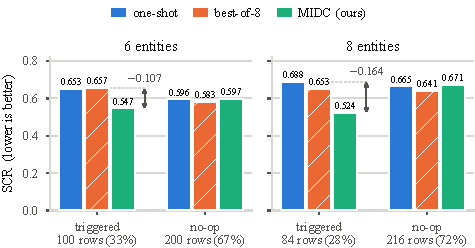
\includegraphics[width=\columnwidth]{figures/gating.pdf}
\caption{Selective correction on FLUX.2-klein-9B, 3 seeds, pooled over $(\text{task},\text{seed})$ rows. ``Triggered'' = at least one correction step accepted. On triggered rows MIDC cuts SCR sharply and beats best-of-8 on the \emph{same} rows; on no-op rows it lands on one-shot, forgoing the small gain best-of-8 buys with $8\times$ compute---a deliberate trade-off, not a free lunch.}
\label{fig:gating}
\end{figure}

Two observations follow. \textbf{First, on the triggered set MIDC cuts SCR sharply and beats best-of-8 on the same rows.} At 8 entities, MIDC vs one-shot is $\Delta{=}{-}0.164$ ($95\%$CI $[-0.207,-0.122]$, $p{<}0.001$, win/tie/loss $57/16/11$) and vs best-of-8 $\Delta{=}{-}0.130$ ($[-0.173,-0.085]$, $p{<}0.001$); at 6 entities, $-0.107$ and $-0.110$ respectively (both $p{<}0.001$). Best-of-8 itself barely beats one-shot here ($-0.034$, $p{=}0.040$ at 8 entities; $+0.003$, $p{=}0.85$ at 6)---scalar re-ranking does not fix the hard cases decomposed diagnosis targets.

\textbf{Second, on the no-op set MIDC is a clean no-op but forgoes best-of-8's small gain.} Against one-shot it is $+0.006$ ($p{=}0.53$) at 8 entities and $+0.001$ ($p{=}0.88$) at 6---no measurable regression against the base. Best-of-8 does buy a small gain there for $8\times$ compute ($-0.024$, $p{=}0.026$ at 8 entities); MIDC declines to act below threshold and forgoes it. Routing no-op rows to best-of-$N$ is an obvious combination we leave to future work.

\paragraph{Correction, not selection.} A skeptic might attribute the gain to scalar selection among MIDC's ${\sim}2$ candidates. The no-op subset rules this out: that output \emph{is} a best-of-2 by verifier total, and its SCR is within $0.006$ of one-shot---selection from 2 candidates buys nothing, while diagnosis plus one correction step buys $0.164$ on the triggered set. The $-0.041$ aggregate is thus a large targeted fix diluted by a deliberate no-op, and the reason the aggregate best-of-8 comparison (\emph{FLUX.2 Scaling}) is not significant.

\subsection{Human Evaluation}
\label{sec:human}

We ran a blind A/B study with 3 labelers over 200 image pairs, judging existence (Q1), identity (Q2), interaction (Q3) and overall quality (Q4) with LEFT/RIGHT/TIE options (Table~\ref{tab:human}).

\begin{table}[ht]
\centering
\small
\setlength{\tabcolsep}{2.5pt}
\caption{Human eval, 3 labelers over 100 pairs per baseline. Win rate is over pairs where at least one labeler expressed a non-tie preference and those preferences were not evenly split, so $n$ is the size of that subset, not the pair count; on Q1 vs.\ UMO all three labelers marked $48$ of $100$ pairs tied. $\kappa>0.2$ is moderate agreement; $\kappa<0$ is disagreement (no claim).}
\label{tab:human}
\begin{tabular}{llcccc}
\toprule
baseline & dim. & win [95\% CI] & $n$ & $\kappa$ & $p$ \\
\midrule
UMO & Q1 exist. & \textbf{0.846 [0.75, 0.94]} & 52 & $+0.32$ & $\mathbf{4{\times}10^{-7}}$ \\
UMO & Q4 overall & 0.589 [0.48, 0.70] & 73 & $+0.15$ & $0.16$ \\
\midrule
best-of-8 & Q1 exist. & 0.500 [0.31, 0.69] & 32 & $+0.48$ & $1.00$ \\
best-of-8 & Q4 overall & 0.523 [0.40, 0.65] & 65 & $+0.17$ & $0.80$ \\
\bottomrule
\end{tabular}
\end{table}

On \textbf{existence (Q1)}, labelers prefer MIDC over the retrained SOTA (UMO) \textbf{84.6\%} of the time ($p{=}4{\times}10^{-7}$, Fleiss $\kappa{=}0.32$ moderate agreement)---the strongest human result and one that directly mirrors the automatic SCR finding that MIDC drops fewer subjects. The result does not depend on how thinly-voted pairs are treated: requiring at least two labelers to express a preference gives $82.9\%$ ($n{=}35$, $p{=}0.0001$) and requiring all three gives $87.0\%$ ($n{=}23$, $p{=}0.0005$). On overall quality (Q4) MIDC is directionally preferred over both baselines but not significantly. Identity (Q2) and interaction (Q3) show negative Fleiss $\kappa$---labelers disagree with each other---so we claim neither, and flag reliable human evaluation of those axes as an open problem.

\section{Discussion and Limitations}
\label{sec:limits}

\paragraph{``Training-free'' is relative to the generator.} MIDC touches no generator weights, but its verifier is LoRA-fine-tuned on 60K pairs of the same task family: strictly, we move training from the generator to the verifier, as best-of-$N$ with a reward model also does. The selling point is \emph{decoupling}---the \emph{same} MIE serves both base models---whereas a retrained generator is bound to one.

\paragraph{The judge is independent of $V$, but not of the loop.} No reported metric comes from the verifier $V$. But SCR and DINO are DINOv2-derived, and MIDC consults DINOv2 per-subject similarity in three places---weak-subject diagnosis, in-portfolio candidate selection, and the acceptance gate---so the loop does partly select on the axis we report, and we should not call the judge independent. Two measurements bound the exposure. \textbf{First}, on the $526$ hard\_4 rows where MIDC accepted nothing, its output is the initial MIE-selected candidate and DINOv2 never influenced it; MIDC still beats UMO there by $+0.030$ DINO ($p{<}0.001$) and $-0.023$ SCR ($p{=}0.022$), so the advantage is not purely self-selection. \textbf{Second}, on the $224$ triggered rows the margin is far larger ($+0.111$ DINO), and there selection-on-the-metric cannot be ruled out from these numbers alone---CLIP-I, which the loop never optimizes, is precisely where MIDC does \emph{not} beat UMO (Table~\ref{tab:main}). The existence conclusion is the one that survives every check, since the human study asks labelers directly and involves neither $V$ nor DINOv2 ($p{=}4{\times}10^{-7}$). An acceptance rule that avoids DINOv2 entirely is the clean fix and the obvious next ablation.

\paragraph{SCR inherits its detector's errors.} Inspecting outputs we find cases---heavy occlusion, near-duplicate subjects---where Grounding-DINO's count disagrees with a human reading, in both directions. These errors apply \emph{identically} to every method, inflating variance rather than biasing any comparison.

\paragraph{When MIDC fails.} Residual failures (Figure~\ref{fig:results}) concentrate on heavy occlusion, where Grounding-DINO itself misses a subject so the diagnosis targets the wrong facet, and on prompts whose spatial language is inherently ambiguous. These are localization and prompt-ambiguity failures rather than routing failures, pointing to stronger open-set detectors and explicit spatial parsing.

\paragraph{Modest absolute gaps.} Even MIDC leaves substantial collapse (SCR ${\approx}0.47$ at 4 entities, $0.63$ at 8): the benchmark is hard and MIDC is a \emph{reducer}, not a solution. The gap to one-shot is consistent and significant on both bases and metrics; the best-of-$N$ comparison is weaker and we do not claim it, being concentrated on the subset MIDC elects to correct (\emph{Selective Correction}). Matching best-of-$N$'s aggregate at half the compute while decisively winning the hard subset is the honest reading. Finally, we compare \emph{one} retrained SOTA on one base; cross-system baselines are future work, and our claim is the diagnostic finding above.


\bibliography{refs}
\end{document}
